%%%%%%%%%%%%%%%%%%%%%%%%%%%%%%%%%%%%%%%%%
% Short Sectioned Assignment
% LaTeX Template
% Version 1.0 (5/5/12)
%
% This template has been downloaded from:
% http://www.LaTeXTemplates.com
%
% Original author:
% Frits Wenneker (http://www.howtotex.com)
%
% License:
% CC BY-NC-SA 3.0 (http://creativecommons.org/licenses/by-nc-sa/3.0/)
%
%%%%%%%%%%%%%%%%%%%%%%%%%%%%%%%%%%%%%%%%%

%----------------------------------------------------------------------------------------
%	PACKAGES AND OTHER DOCUMENT CONFIGURATIONS
%----------------------------------------------------------------------------------------

\documentclass[paper=a4, fontsize=11pt]{scrartcl} % A4 paper and 11pt font size

\usepackage[T1]{fontenc} % Use 8-bit encoding that has 256 glyphs
\usepackage{fourier} % Use the Adobe Utopia font for the document - comment this line to return to the LaTeX default
\usepackage[english]{babel} % English language/hyphenation
\usepackage{amsmath,amsfonts,amsthm} % Math packages

\usepackage{lipsum} % Used for inserting dummy 'Lorem ipsum' text into the template

\usepackage{sectsty} % Allows customizing section commands
\allsectionsfont{\centering \normalfont\scshape} % Make all sections centered, the default font and small caps

\usepackage{graphicx}
\usepackage{float}

\usepackage{fancyhdr} % Custom headers and footers
\pagestyle{fancyplain} % Makes all pages in the document conform to the custom headers and footers
\fancyhead{} % No page header - if you want one, create it in the same way as the footers below
\fancyfoot[L]{} % Empty left footer
\fancyfoot[C]{} % Empty center footer
\fancyfoot[R]{\thepage} % Page numbering for right footer
\renewcommand{\headrulewidth}{0pt} % Remove header underlines
\renewcommand{\footrulewidth}{0pt} % Remove footer underlines
\setlength{\headheight}{13.6pt} % Customize the height of the header

\numberwithin{equation}{section} % Number equations within sections (i.e. 1.1, 1.2, 2.1, 2.2 instead of 1, 2, 3, 4)
\numberwithin{figure}{section} % Number figures within sections (i.e. 1.1, 1.2, 2.1, 2.2 instead of 1, 2, 3, 4)
\numberwithin{table}{section} % Number tables within sections (i.e. 1.1, 1.2, 2.1, 2.2 instead of 1, 2, 3, 4)

\setlength\parindent{0pt} % Removes all indentation from paragraphs - comment this line for an assignment with lots of text


%----------------------------------------------------------------------------------------
%	TITLE SECTION
%----------------------------------------------------------------------------------------

\newcommand{\horrule}[1]{\rule{\linewidth}{#1}} % Create horizontal rule command with 1 argument of height

\title{
\normalfont \normalsize
\textsc{McGill University} \\ [25pt] % Your university, school and/or department name(s)
\horrule{0.5pt} \\[0.4cm] % Thin top horizontal rule
\huge Assignment 1 \\ % The assignment title
\horrule{2pt} \\[0.5cm] % Thick bottom horizontal rule
}

\author{
    Nabil Chowdhury \\
    \small{ID: 260622155} \\
    \small{COMP 551}
} % Your name

\date{\normalsize\today} % Today's date or a custom date

\begin{document}

\maketitle % Print the title

%--------------
%	PROBLEM 1
%--------------

\section{Model Selection}
%--------------
\subsection{Fitting 20-degree polynomial to the dataset}
Dataset-1 consists of a real-valued scalar as input, and a real-valued scalar as output. In order to fit a 20 degree polynomial, we must create features \textit{x\textsuperscript{2}, x\textsuperscript{3},..., x\textsuperscript{20}}, since \textit{x\textsuperscript{1}} is already given to us. We must also include \textit{x\textsuperscript{0} = 1} in the input (the bias term). We must find \textit{w\textsubscript{0}, w\textsubscript{1},..., w\textsubscript{20}} such that \textit{\^{y} = w\textsubscript{0} + w\textsubscript{1}x\textsuperscript{1} + ... + w\textsubscript{20}x\textsuperscript{20}}, where \^{y} is the prediction. \\

Applying the closed form solution  \(w = (X^TX)^{-1}X^Ty\) yields the least-squares weights \textit{w} for the polynomial. Using these weights, the following mean-squared-errors for the training, validation and test sets were calculated:

\begin{center}
\begin{tabular}{ |c|c| }
	\hline
	\textbf{Set} & \textbf{MSE} \\
	\hline
	Train & 7.15259 \\
	Valid & 458.64632 \\
	Test & 17.25163 \\
	\hline
\end{tabular}
\end{center}

Here is the fit on the training, validation, and test sets:
\begin{figure}[H]
    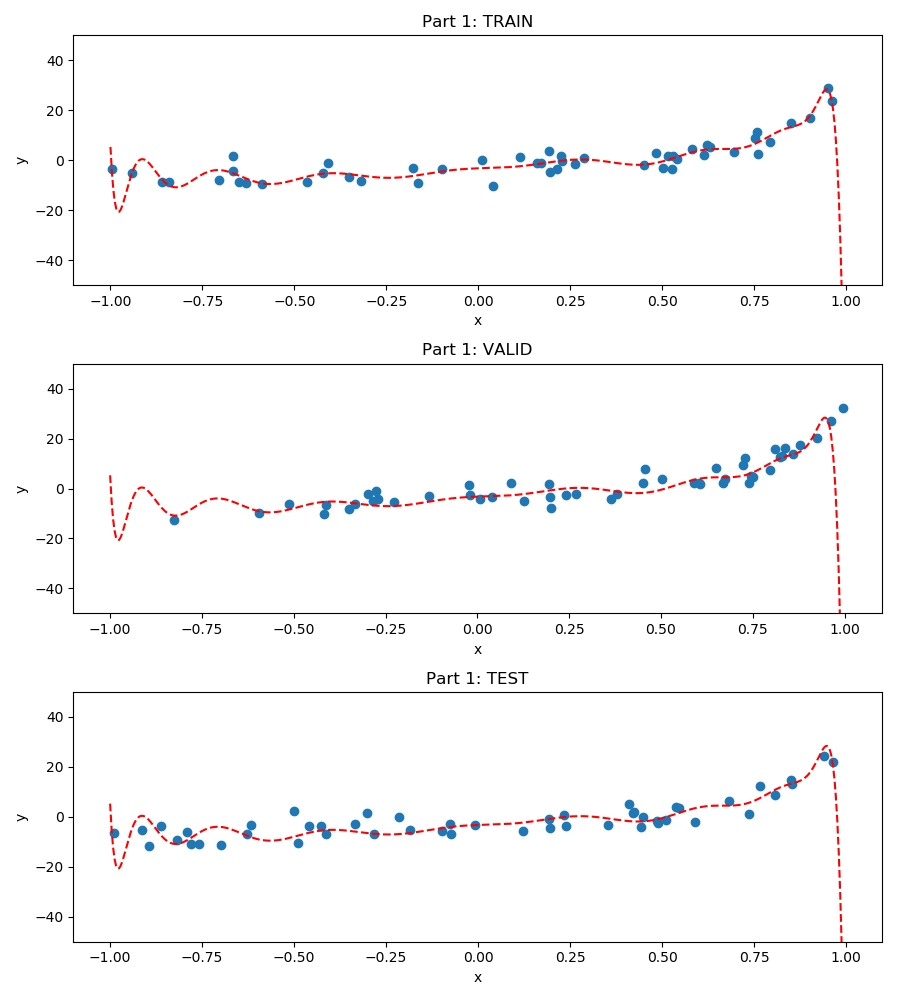
\includegraphics[width=\linewidth]{q1p1.png}
    \caption{Fit of 20-degree polynomial without regularization}
    \label{fig:q1p1}
\end{figure}


A closer look at the training plot shows oscillations in the fit (i.e. it is trying very hard to fit the training data). This observation, along with a high validation MSE of 458.64632 indicates that the 20-degree polynomial overfits the dataset. In other words, while the training MSE is low, the curve does not generalize well to the validation set.

\begin{figure}[H]
    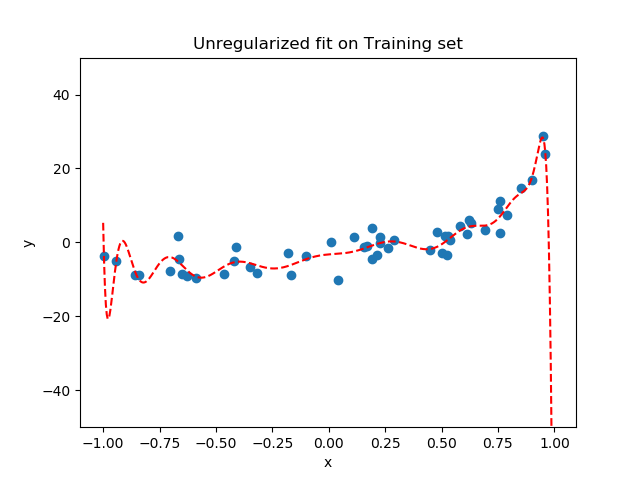
\includegraphics[width=\linewidth]{q1p12.png}
    \caption{Fits training set well}
    \label{fig:q1p12}
    \vspace{0.5cm}
    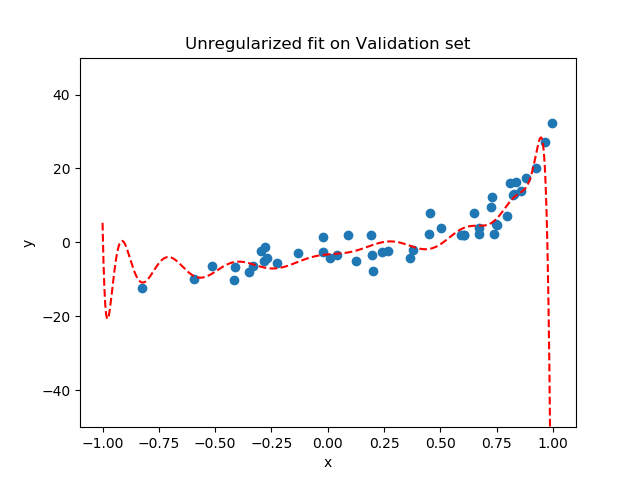
\includegraphics[width=\linewidth]{q1p13.png}
    \caption{Fit does not generalize well to validation set}
    \label{fig:q1p13}
\end{figure}

\subsection{Adding L2 regularization to the model}
Adding L2 regularization to our model requires changing the closed form solution by adding a \( \lambda I \) term to \(X^TX\) as follows:
\[ w = (X^TX + \lambda I)^{-1}X^Ty \]

Varying \(\lambda\) from 0 to 1 with increments of .0001 yields the following results for the training and validation sets:

\begin{figure}[H]
    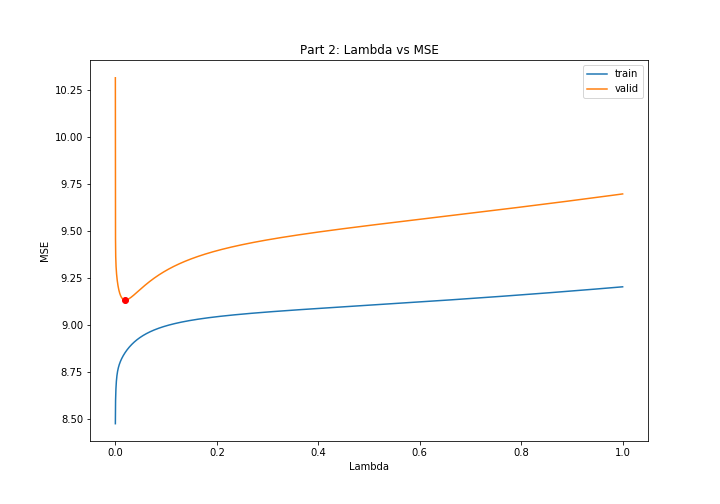
\includegraphics[width=\linewidth]{q1p14.png}
    \caption{\(\lambda\) vs MSE for training and validation sets}
    \label{fig:q1p14}
\end{figure}

The optimum \(\lambda\), based on the lowest MSE of the validation set is 0.0197. Retraining the model with this chosen lambda yields much better MSEs for the validation and test sets:

\begin{center}
\begin{tabular}{ |c|c| }
	\hline
	\textbf{Set} & \textbf{MSE with \(\lambda = 0.0197\)} \\
	\hline
    Train & 8.85645 \\
	Valid & 9.13508 \\
	Test & 10.73230 \\
	\hline
\end{tabular}
\end{center}

We can also visualize this regularized fit on the training, validation and test sets:

\begin{figure}[H]
    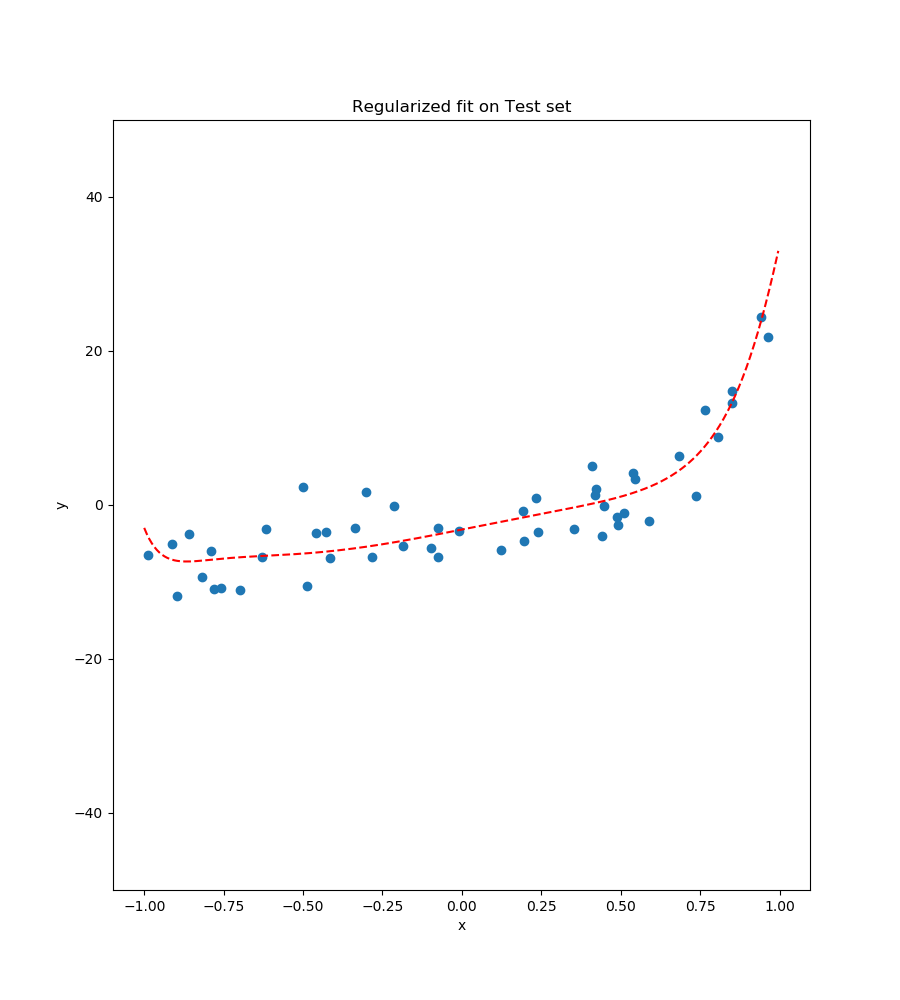
\includegraphics[width=\linewidth]{q1p15.png}
    \caption{Fit of 20-degree polynomial on training set with optimal lambda}
    \label{fig:q1p15}
    \vspace{0.5cm}
    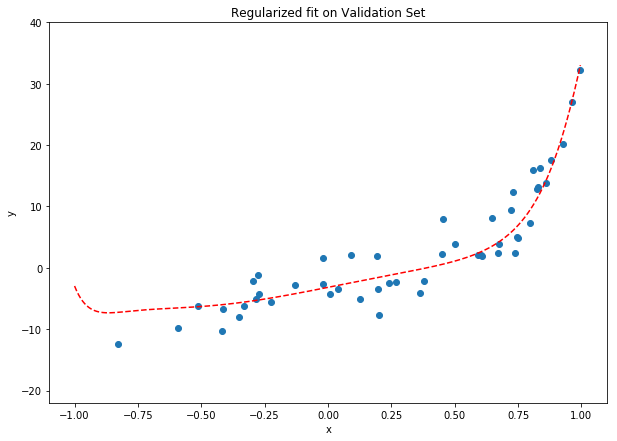
\includegraphics[width=\linewidth]{q1p16.png}
    \caption{Fit of 20-degree polynomial on validation set with optimal lambda}
    \label{fig:q1p16}
\end{figure}
\begin{figure}[H]
    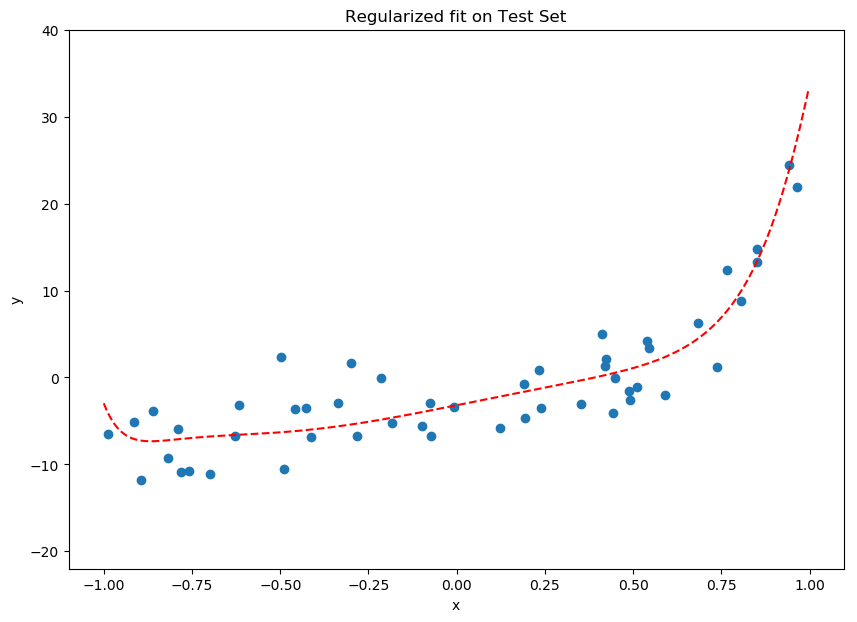
\includegraphics[width=\linewidth]{q1p17.png}
    \caption{Fit of 20-degree polynomial on test set with optimal lambda}
    \label{fig:q1p17}
\end{figure}

\subsection{Estimation of degree of source polynomial}

Observing the regularized fit of the model indicates two sharp bends (at the ends), with approximately 3 slight bends in between. This indicates that a 6\textsuperscript{th} degree polynomial is a good estimate of the source polynomial.

%--------------
%	PROBLEM 2
%--------------

\section{Gradient Descent For Regression}
%--------------
\subsection{Fitting a linear regression model using Stochastic Gradient Descent}

Dataset-2 provides us with a real-valued scalar as input and a real-valued scalar as output. Using Stochastic Gradient Descent (SGD) with a step size \(\alpha\) of \(10^{-6}\) yields the following learning curve (Note: since the weights are randomly initialized, this will not be the exact curve for every run of the code in the Jupyter Notebook):

\begin{figure}[H]
    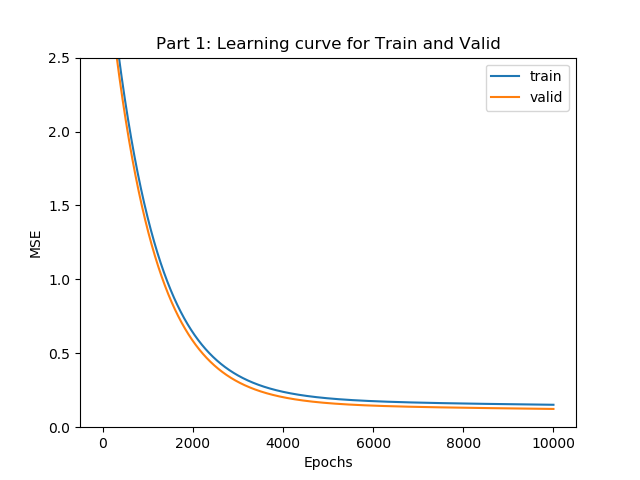
\includegraphics[width=\linewidth]{q2p1.png}
    \caption{Epoch vs MSE at \(\alpha=10^{-6}\)}
    \label{fig:q2p1}
\end{figure}
\begin{center}
\begin{tabular}{ |c|c| }
	\hline
	\textbf{Set} & \textbf{Final MSE at \(\alpha = 10^{-6}\)} \\
	\hline
    Train & 0.10277 \\
	Valid & 0.07558 \\
	Test & 0.08120 \\
	\hline
\end{tabular}
\end{center}

\subsection{Finding the best step size}
The following step sizes were tested to determine which step size yielded the best results for the validation set:  \(10^{-6}, 5\times10^{-6}, 10^{-5}, 5\times10^{-5}, 10^{-4}, 5\times10^{-4}, 10^{-3}, 5\times10^{-3}, 10^{-2}, 5\times10^{-2}\). Based on these values and the initial random weights used in 2.1, the best \(\alpha\) was found to be \(5\times10^{-6}\).

\begin{figure}[H]
    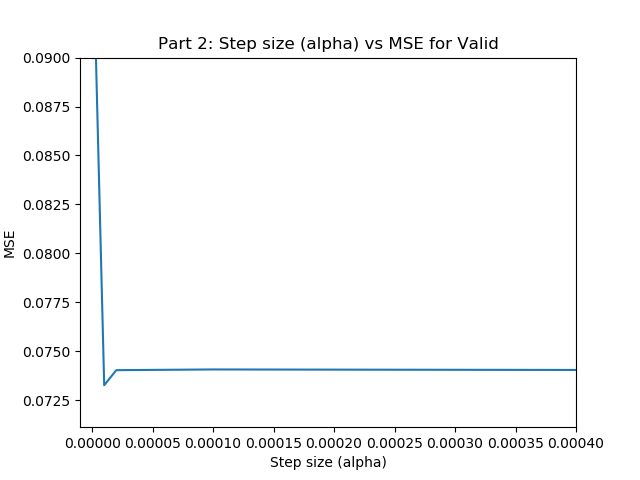
\includegraphics[width=\linewidth]{q2p2.png}
    \caption{\(\alpha\) vs MSE for the Validation set}
    \label{fig:q2p2}
\end{figure}

The MSE for all three sets using the optimal \(\alpha\) value of \(5\times10^{-6}\) is:
\begin{center}
\begin{tabular}{ |c|c| }
	\hline
	\textbf{Set} & \textbf{Final MSE at \(\alpha = 5\times10^{-6}\)} \\
	\hline
    Train &  0.09606 \\
	Valid & 0.07289 \\
	Test & 0.07099 \\
	\hline
\end{tabular}
\end{center}
As we can see, the MSEs at \(\alpha = 5\times10^{-6}\) are lower than at  \(\alpha = 10^{-6}\)

\subsection{Evolution of the regression fit during training}
The following figures show the progression of SGD at 0, 800, 1600, 2400, 3200 and 4000 epochs (using \(\alpha\ = 5\times10^{-6}\)).

\begin{figure}[H]
    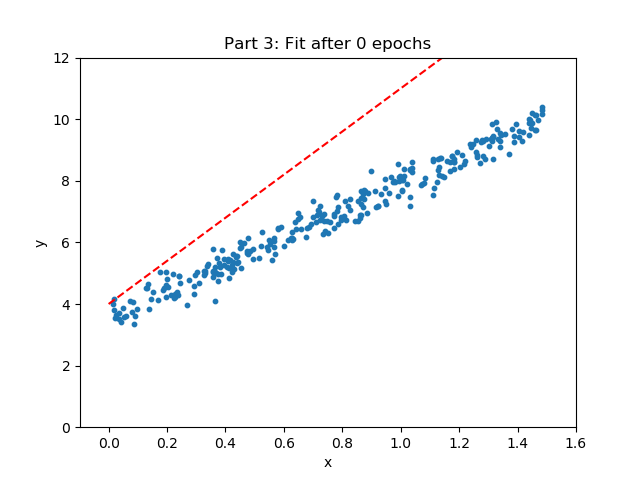
\includegraphics[width=\linewidth]{q2p31.png}
    \caption{Fit with randomly initialized weights}
    \label{fig:q2p31}
    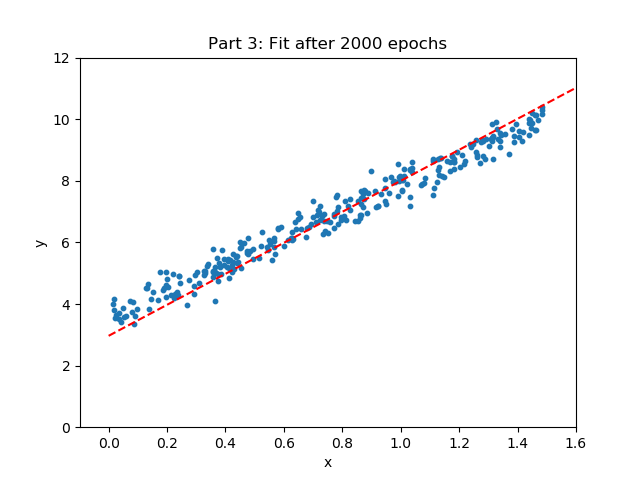
\includegraphics[width=\linewidth]{q2p32.png}
    \caption{SGD makes large jump towards optimum weights}
    \label{fig:q2p32}
\end{figure}
\begin{figure}[H]
    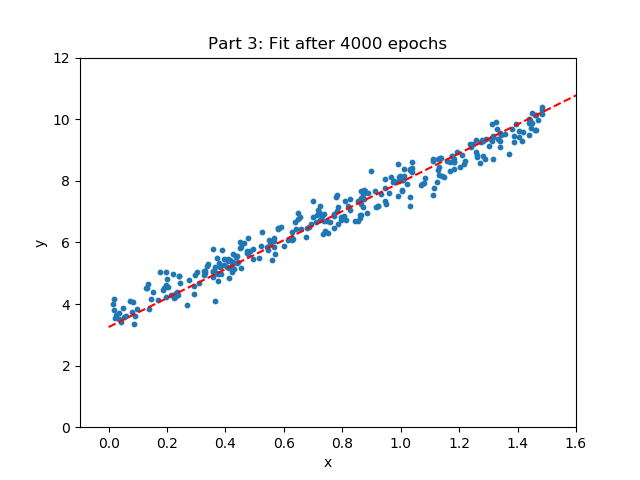
\includegraphics[width=\linewidth]{q2p33.png}
    \caption{SGD starts taking smaller steps towards optimum}
    \label{fig:q2p33}
    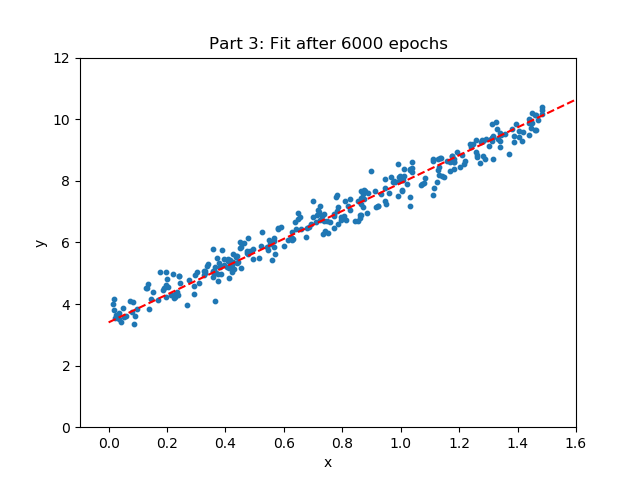
\includegraphics[width=\linewidth]{q2p34.png}
    \caption{At 6000 epochs}
    \label{fig:q2p34}
\end{figure}
\begin{figure}[H]
    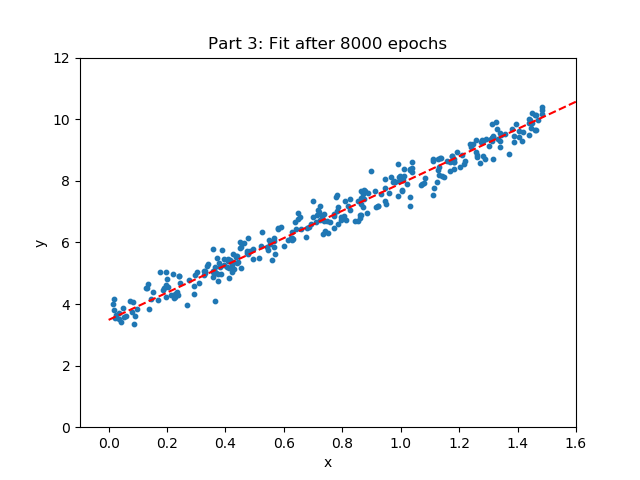
\includegraphics[width=\linewidth]{q2p35.png}
    \caption{Near the end of training}
    \label{fig:q2p35}
    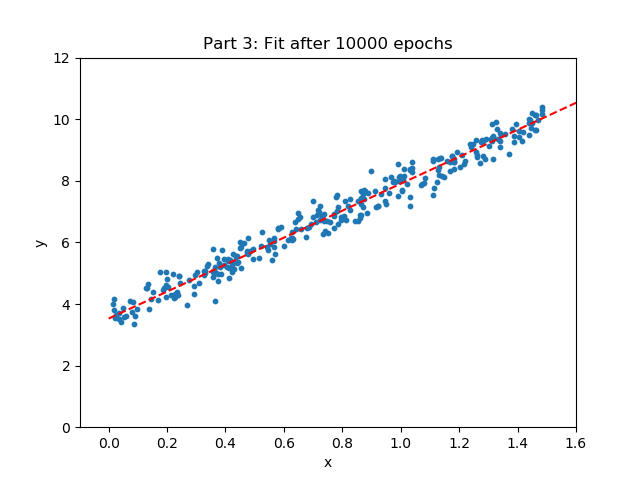
\includegraphics[width=\linewidth]{q2p36.png}
    \caption{End of training}
    \label{fig:q2p36}
\end{figure}

\section{Real-life dataset}
\subsection{Fill in missing values}
The mean is a good filler for missing values if that particular attribute is interval or ratio data. Interval data is data that has a definite order and an exact difference, such as temperature. Ratio data is data with an absolutely defined zero, such as the Kelvin scale for temperature. In our case, the attributes are numerical data and thus is a good fit for the mean. The median and mode can also be used on such data. \\

The mean will not work categorical data since categories may not have an exact order (nominal data), and if they do, the distance between subsequent categories may not be definite (ordinal data). For nominal data, the mode is a good candidate for filling in missing values whereas for ordinal data, both the mode and median can be used, since there is notion of order and distance, even though the distance is not exactly known. \\

For this dataset, the mean of each feature (over all examples) was used to fill in missing values.

\subsection{Fitting the model}
The data contained 127 attributes, of which the first five were "not predictive" according to the source, and therefore omitted. Including the bias column added to the dataset, a total of 123 weights were used in the model. The data was shuffled and split into five 80-20 train-test splits. Using both the closed form solution and gradient descent separately on each of the splits, the following MSEs averaged over 5 splits were found:\\

Note: The MSE depends on the random shuffling of the data. This is one result.
\begin{center}
\begin{tabular}{ |c|c| }
	\hline
	\textbf{Algorithm} & \textbf{MSE on test} \\
	\hline
    Closed form solution & 0.11375 \\
	Gradient descent & 0.45150 \\
	\hline
\end{tabular}
\end{center}

The weights for each fold calculated by both the closed form and gradient descent are attached in the csv files \texttt{weights\_for\_closed\_form} and \texttt{weights\_for\_gradient\_descent} respectively. Each column represents the weights calculated for each fold.

\subsection{Ridge Regression}
For this part, only the closed form solution was used, but the code in the Jupyter Notebook supports Ridge Regression for gradient descent as well. \\

Values of \(\lambda\) between 0 and 5, with increments of 0.05 were tested to find the best \(\lambda\). Again, since the examples are shuffled initially, this value will change from one execution of the code to another. For the shuffle order used for 3.2, the best \(\lambda\) is 1.45, with an average MSE across the five folds (on test set) of 0.01841. This is an improvement from the test MSEs in 3.2. \\

Here is a graph of \(\lambda\) vs MSE:
\begin{figure}[H]
    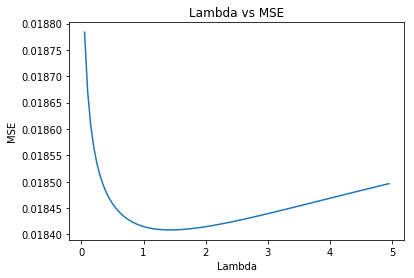
\includegraphics[width=\linewidth]{q3p31.png}
    \caption{\(\lambda\) vs average MSE on test set}
    \label{fig:q3p31}
\end{figure}

Using the optimal weights produced by \(\lambda = 1.45\), we can relate Ridge Regression to the importance of certain weights. Weights with magnitudes close to zero contribute less to the prediction than weights with larger magnitudes. By retraining the model with regularization using \(\lambda = 1.45\) and sorting the weights by magnitude, we can observe which weights contribute the least (this was done for each of the five folds and then aggregated). Please see the Jupyter Notebook for implementation details. For this particular run, the number of features dropped by the algorithm was 51, producing a better MSE of 0.01792:

\begin{center}
\begin{tabular}{ |c|c| }
	\hline
	\textbf{No. of features} & \textbf{MSE on test, with \(\lambda = 1.45\)} \\
	\hline
    All & 0.01841 \\
	\textbf{72} &  \textbf{0.01792} \\
	\hline
\end{tabular}
\end{center}

\newpage

\begin{thebibliography}{9}
\bibitem{discussions}
For Question 1.1: Helped the following people with understanding the problem statement and answering Python-related questions: John Wu, Tiffany Wang, Frank Ye. All code and writing is original and written individually.

\bibitem{fillingmissingdata}
For Question 3.1: http://www.mymarketresearchmethods.com/types-of-data-nominal-ordinal-interval-ratio/

\bibitem{featureselection}
For Question 3.3: http://blog.datadive.net/selecting-good-features-part-ii-linear-models-and-regularization/
\end{thebibliography}

\end{document}
